\section{Daemon}


\begin{frame}
  \frametitle{Zweck}
  \begin{itemize}
   \item \textit{Lxc} benötigen root-Rechte
   \item Nutzung sollte idealerweise unprivilegiert ablaufen
   \item Erstellung und Verwaltung durch einen \textit{daemon}
  \end{itemize}
\end{frame}


\begin{frame}[fragile]
 \frametitle{Daemon Design}
 \begin{itemize}
  \item Kommunikation via Socket (Unix Domain Socket)
  \item Zugriffskontrolle über Berechtigung
  \item request:\\\begin{verbatim}
	{"action": "run_prog"
	 "b64_data": program
	 "timeout": 60}
        \end{verbatim}

  \item Daemon benutzt eigenes Konfigurations-Template
  \begin{itemize}
   \item Cgroup Limits
   \item Alle Kernel Capabilities ablegen
   \item Mountpoints
  \end{itemize}
  \item Erstellt Debian Container
 \end{itemize}
\end{frame}


\begin{frame}
 \frametitle{Workflow}
 \begin{center}
  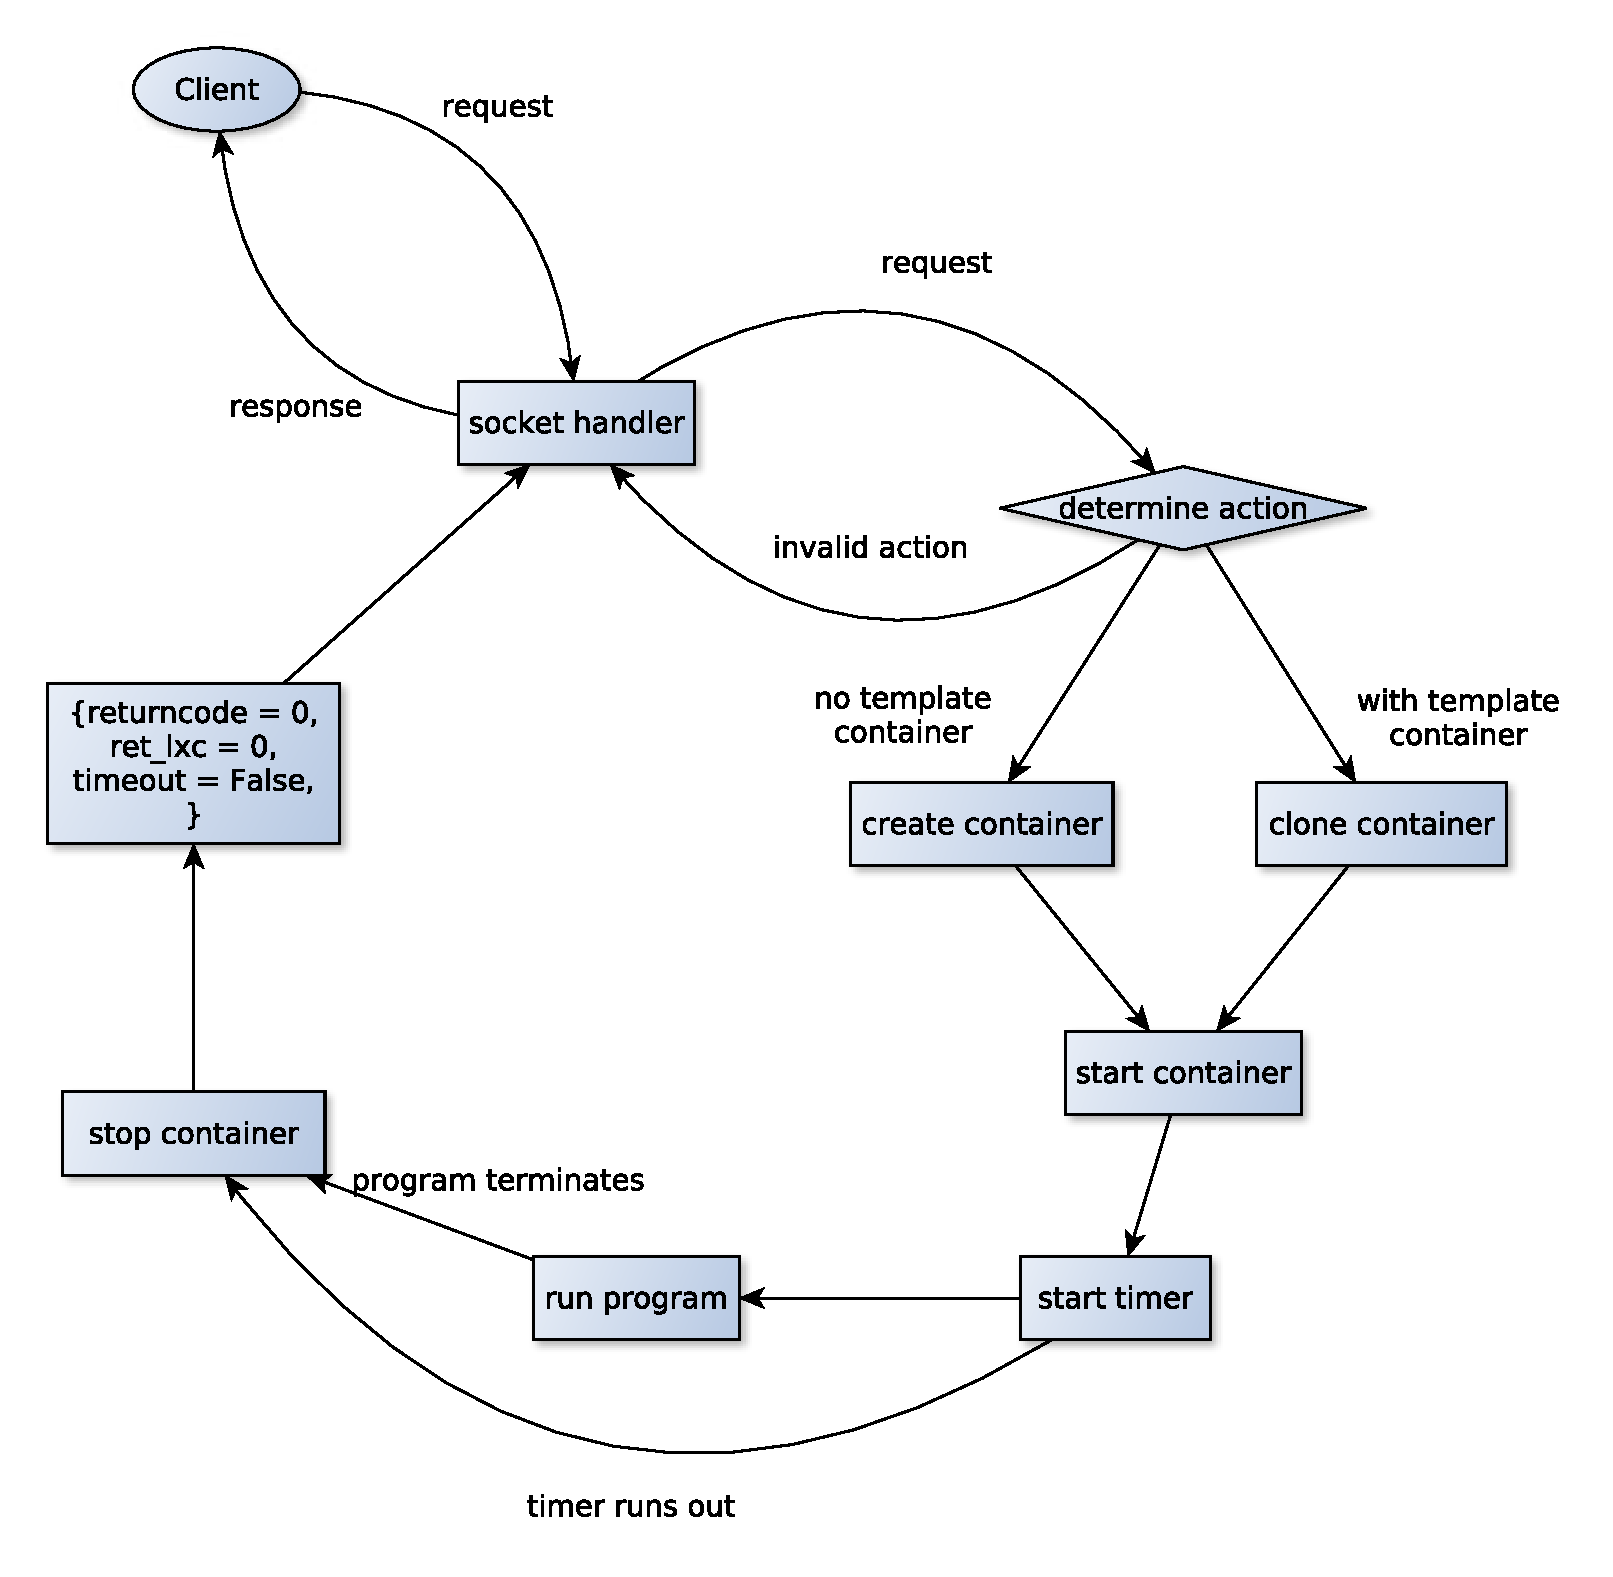
\includegraphics[width=0.7\textwidth]{fig/workflow}
 \end{center}
\end{frame}

\section{Probleme}

\begin{frame}
 \frametitle{Probleme}
 \begin{itemize}
  \item Umstrukturierung der Konfigurationsdateien
  \begin{itemize}
   \item Auslagerung von Sektionen in allgemeine Konfigurationen
   \item Änderungen an der Mountpoint Syntax
  \end{itemize}
  \item Änderungen am Rückgabewert des ausgeführten Programmes
  \item Fehlen von Kernel Modulen in Arch Linux:
  \begin{itemize}
   \item User Namespace (Befürchtung kritischer Bugs)
   \item Cgroups: Kernel Memory Extension (Memory Reclaim fehlt)
  \end{itemize}
 \end{itemize}
\end{frame}

\begin{frame}[fragile]
 \frametitle{Bug im Python Language Binding}
 \begin{itemize}
  \item API greift auf C-Funktionen zu
  \item Global Interpreter Lock
  \begin{itemize}
   \item blockt alle anderen Threads beim Ausführen einer externen C-Funktion
  \end{itemize}
  \item Timer-Thread geblockt während Programmausführung
 \end{itemize}
 Patch:
 \begin{verbatim}
       if (wait) {
+        Py_BEGIN_ALLOW_THREADS
         ret = lxc_wait_for_pid_status(pid);
+        Py_END_ALLOW_THREADS
         /* handle case where attach fails */
         if (WIFEXITED(ret) && WEXITSTATUS(ret) == 255)
             ret = -1;
 \end{verbatim}
\end{frame}
